\begin{frame}{Strong stripes change which digits cluster together}
\centering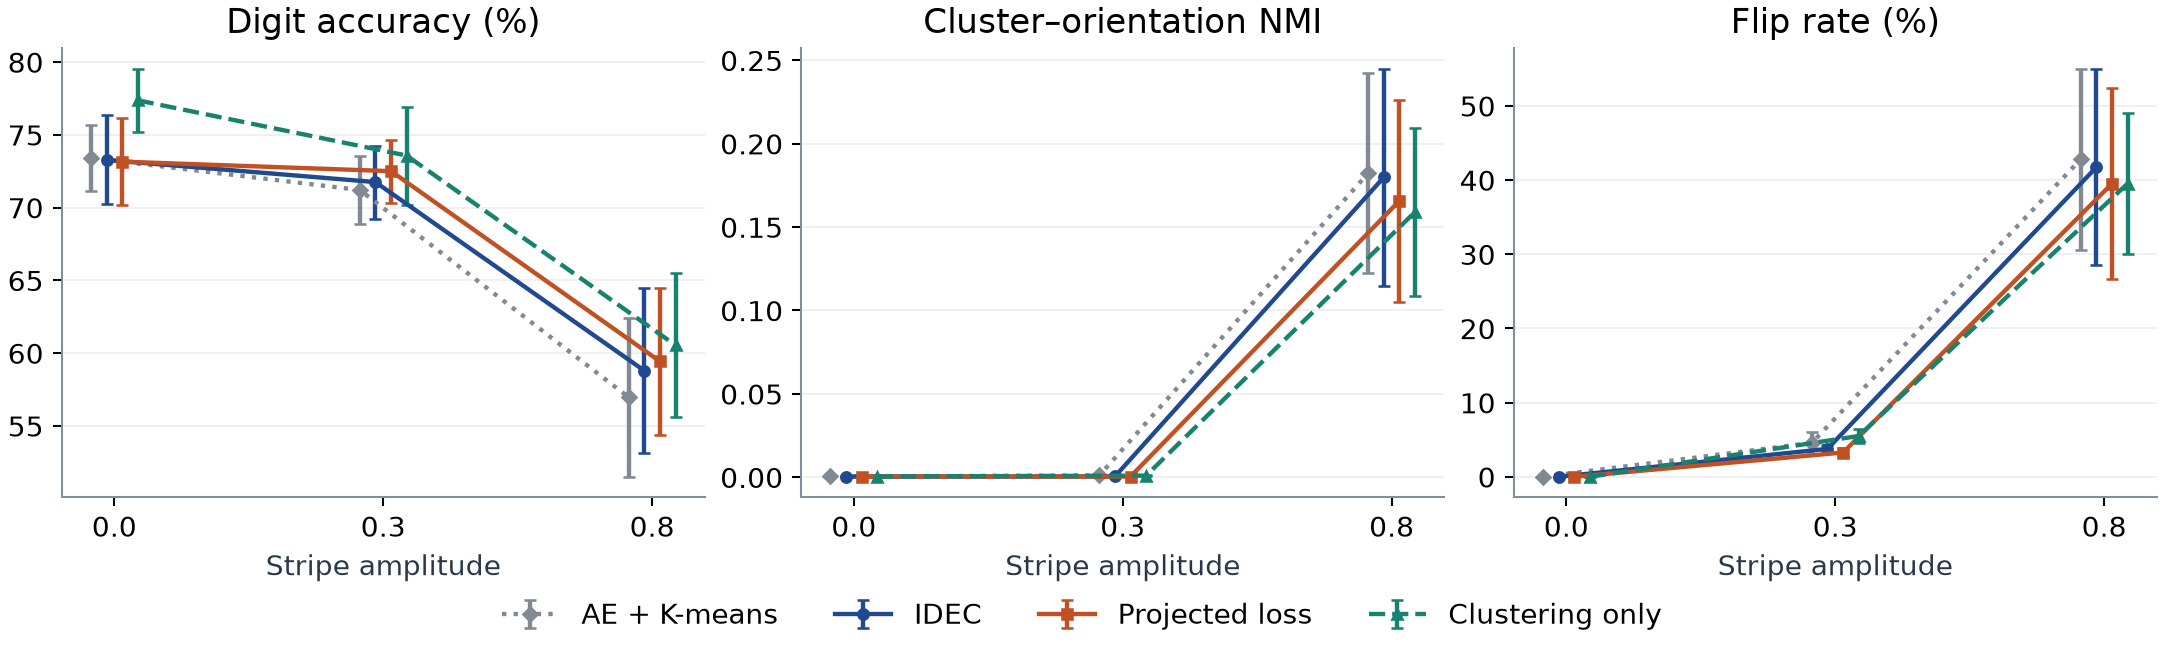
\includegraphics[width=.97\linewidth]{../figures/outcomes.png}
\notefoot{Dots are five-seed means and whiskers span one sample standard deviation. The flip rate holds the digit fixed and reverses the stripe orientation.}
\end{frame}

\begin{frame}{Paired runs show how much the loss changes accuracy}
\centering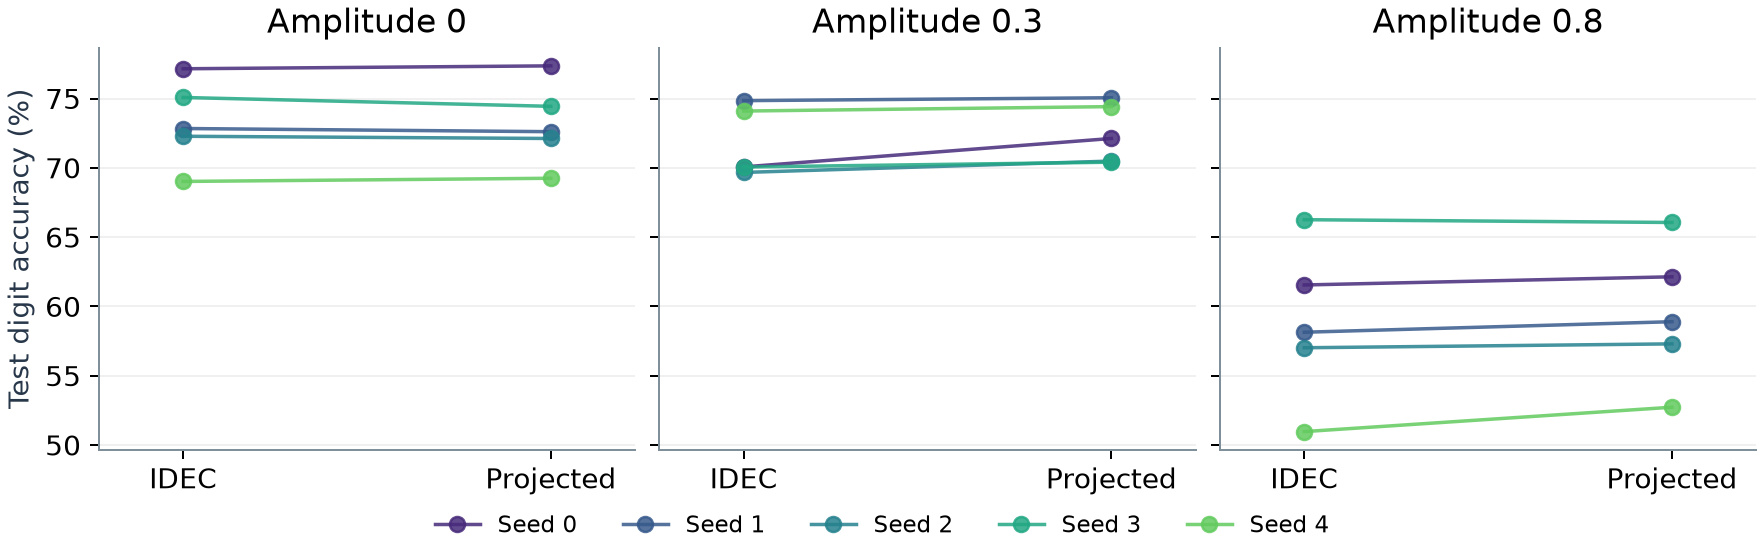
\includegraphics[width=.87\linewidth,height=.55\textheight,keepaspectratio]{../figures/paired.png}
\notefoot{At strong amplitude, digit ACC improved for four of five seeds. The paired mean improvement was 0.64 percentage points (sample SD 0.73). One seed lost 0.20 points.
}
\end{frame}

\begin{frame}{At which training stage do the clusters become sensitive?}
Before any IDEC updates, 42.79\% of digits changed cluster when the stripes switched. We tested this observation by changing pretraining and fine-tuning independently.
\par\medskip
\key{Share of test digits that switch clusters under strong stripes}
\begin{center}\small
\begin{tabular}{lrrr}
\toprule
 & Before & \multicolumn{2}{c}{After fine-tuning}\\
\cmidrule(lr){3-4}
Pretraining & fine-tuning & Full pixel & Projected\\
\midrule
Full pixel & 42.79\% & 42.22\% & 39.53\%\\
Projected & 1.83\% & 4.73\% & 2.61\%\\
\bottomrule
\end{tabular}

\end{center}
\notefoot{Follow-up designed after the main experiment. All four combinations were trained again on the same data with five paired seeds. Each row forks one initialization per seed.}
\end{frame}

\begin{frame}{What the stripe experiment tells us about IDEC}
\begin{columns}[T,onlytextwidth]
\column{.47\textwidth}
\key{The change helped modestly}\par\medskip
At strong amplitude, flip rate fell from \textbf{41.72\% to 39.50\%}. All five seeds became less sensitive. Accuracy rose from 58.79\% to 59.43\%.
\column{.47\textwidth}
\key{Sensitivity began earlier}\par\medskip
Before IDEC fine-tuning, AE + K-means already flipped on \textbf{42.79\%} of digits. Even the clustering-only arm flipped on 39.51\%.
\end{columns}
\vspace{7mm}
A next experiment would change reconstruction during pretraining and fine-tuning separately to isolate when orientation enters the partition.
\notefoot{One dataset, a known synthetic nuisance, five model seeds and a fixed budget. The template removes one reconstruction penalty while leaving the encoder input intact.}

\end{frame}
